% Nallino, Part II p. 239: Ptolemy's model of the longitudes of the superior planets and Venus, redrawn from the
% print at the size of the print. The coordinates are those of a 400 dpi render of the figure (crop from x 338 pt,
% y 236 pt of the master page; y downward). The deferent has its centre in M, the equant circle (of the same
% diameter) in E'; E is the centre of the Earth, G and K the apogee and the perigee of the excentric, H the centre of
% the epicycle; E'HQ and EHP are the lines from the centre of the equant and from the Earth through H.
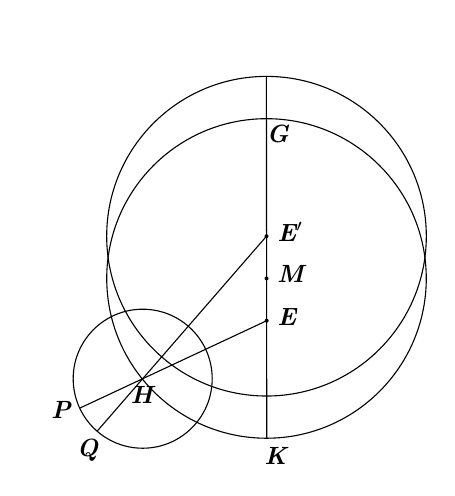
\begin{tikzpicture}[x=0.0635mm,y=-0.0635mm,line width=0.4pt,every node/.style={font=\bfseries\itshape\small,inner sep=1pt}]
\path (0,-8);
\coordinate (Ep) at (477.6,409);
\coordinate (M) at (477.6,493.5);
\coordinate (E) at (478,578);
\coordinate (H) at (230,694);
\coordinate (P) at (104.1,752.9);
\coordinate (Q) at (138.9,798.9);
\draw (Ep) circle[radius=319.6];
\draw (M) circle[radius=319.5];
\draw (H) circle[radius=139];
\draw (477.4,89.5) -- (478.1,813);
\draw (Ep) -- (Q);
\draw (E) -- (P);
\fill (Ep) circle[radius=4];
\fill (M) circle[radius=4];
\fill (E) circle[radius=4];
\node at (500,204) {G};
\node at (518,400) {E\rlap{$'$}};
\node at (525.5,485) {M};
\node at (518,570.5) {E};
\node at (228,727) {H};
\node at (66.5,756.5) {P};
\node at (119.5,837.5) {Q};
\node at (495.5,849) {K};
\end{tikzpicture}
